\documentclass{article}

\usepackage{geometry}
\usepackage{fancyhdr}
\usepackage{graphicx}
\usepackage[a]{esvect}
\usepackage[T1]{fontenc}
\usepackage[hidelinks]{hyperref}
\usepackage{setspace}
\usepackage{logicDG, calcDG}
\usepackage{amsfonts}
\usepackage{siunitx}
\sisetup{per-mode=symbol}
\usepackage[spanish, es-noshorthands, es-noquoting]{babel}
\usepackage{pgfplots}
\pgfplotsset{compat = newest}
\usetikzlibrary{angles, quotes, patterns}
\usepackage{marginnote}


\pagestyle{fancy}
\fancyhf{}
\setlength{\headheight}{70.38103pt}

% ~~~~~~ Autor/es y Título Esquina ~~~~~~ %
\rhead{\textit{David G., Laura R. Luisa R., María V.}}
\rfoot{Lab. Rendija ancha}
% ~~~~~~ Autor/es y Título Esquina ~~~~~~ %

\lhead{\includegraphics[width = 4cm]{\logo}}
\lfoot{Página \thepage}

\renewcommand{\headrule}{\hbox to \headwidth{\color{rojoEci}\leaders\hrule height \headrulewidth\hfill}}
\renewcommand{\footrulewidth}{0.4pt}

\hyphenpenalty=10000

\newcommand{\logo}{"C:/Users/usuario/OneDrive/Documentos/U/logo-eci.png"}

% ~~~~~~ Autor/es y Titulo ~~~~~~ %
\newcommand{\titlename}{Laboratorio de Rendija Ancha}
\renewcommand{\author}{{David Gómez, Laura Rincón, Luisa Rodríguez, María Vivas}}
% ~~~~~~ Autor/es y Titulo ~~~~~~ %

\definecolor{rojoEci}{RGB}{225, 70, 49}



% Enumi func

\renewcommand{\labelenumi}{(\Roman{enumi})}
\renewcommand{\labelenumii}{(\roman{enumii})}

\doublespacing
\begin{document}
\begin{titlepage}
    \begin{center}
        \vspace{1cm}

        \textbf{\Huge{\titlename}}

        \vspace{1.5cm}

        \textbf{\large{\author}}

        \vspace{3cm}

        \includegraphics[width=0.8\textwidth]{\logo}
        
        \vfill

        Física de Calor y Ondas

        Escuela Colombiana de Ingeniería Julio Garavito

        \today
    \end{center}
\end{titlepage}

\clearpage
\tableofcontents

\section{Introducción}

Cuando se tiene una rendija ancha, y se hace insidir un frente de onda plano,
    provoca que cada punto del frente de onda sea un emisor isotrópico de ondas,
    cuyo efecto neto es la superposición de todas las ondas que llegan a un punto p.

    Recordemos que la condición de interferencia constructiva está 
dada, bajo la condiciónde que $\theta \approx 0$, entonces:
Cuando $a\sin(\theta) \approx a\tan(\theta)$:
\[
    Y_{n,\max} = \frac{L_0\lambda}{a} \left(n + \frac{1}{2}\right)
\]

Para el experimento se hizo atravesar una luz lacer a traves de una rendija de cierto grosor hasta llegar a un lector que medía la intensidad de la luz en diversos ángulos. El lector estaba sincronizado a un programa que interpreta los datos y los grafica.

La medición que se hizo fue la de la intensidad de la luz al hacerla pasar por varias rendijas de diversos grosores en posiciones distintas, además de calcular la intensidad máxima tanto manualmente como con los datos del programa

\section{Datos tomados}

\newcolumntype{C}{>{$}c<{$}}
\begin{enumerate}
    \item Rendija de \qty{0.04}{\mm}
    

\setlength{\tabcolsep}{5pt}
\RenewDocumentCommand{\arraystretch}{}{1.2}
    \begin{tabular}{|C|C|}
        \hline
        \text{Intensidad} (\%)  & \text{Posición} (\si{\mm})\\
        \hline
        15.007019043    & -35.0096659775    \\
        15.4052734375   & -36.2796659525    \\
        16.5725708008   & -37.6343325925    \\
        19.1329956055   & -38.9889992325    \\
        22.4639892578   & -40.3436658725    \\
        25.0244140625   & -41.740665845     \\
        27.0874023438   & -43.0529991525    \\
        29.573059082    & -44.3229991275    \\
        33.0032348633   & -45.5929991025    \\
        38.0996704102   & -47.0323324075    \\
        43.9895629883   & -48.4716657125    \\
        47.3449707031   & -49.8263323525    \\
        \hline
    \end{tabular}
    \hspace{10pt}
    \begin{tabular}{|C|C|}
        \hline
        \text{Intensidad} (\%)  & \text{Posición} (\si{\mm})\\
        \hline
        46.2020874023   & -51.13866566      \\
        41.8273925781   & -52.4933323       \\
        36.3342285156   & -53.84799894      \\
        31.1645507812   & -55.20266558      \\
        26.6403198242   & -56.5996655525    \\
        23.0102539062   & -57.996665525     \\
        20.0286865234   & -59.3936654975    \\
        17.7917480469   & -60.79066547      \\
        16.2506103516   & -62.1876654425    \\
        15.4052734375   & -63.584665415     \\
        15.1062011719   & -65.02399872      \\
        \hline
    \end{tabular}

    $2Y_0 = \qty{30,0143327425}{\mm}$

    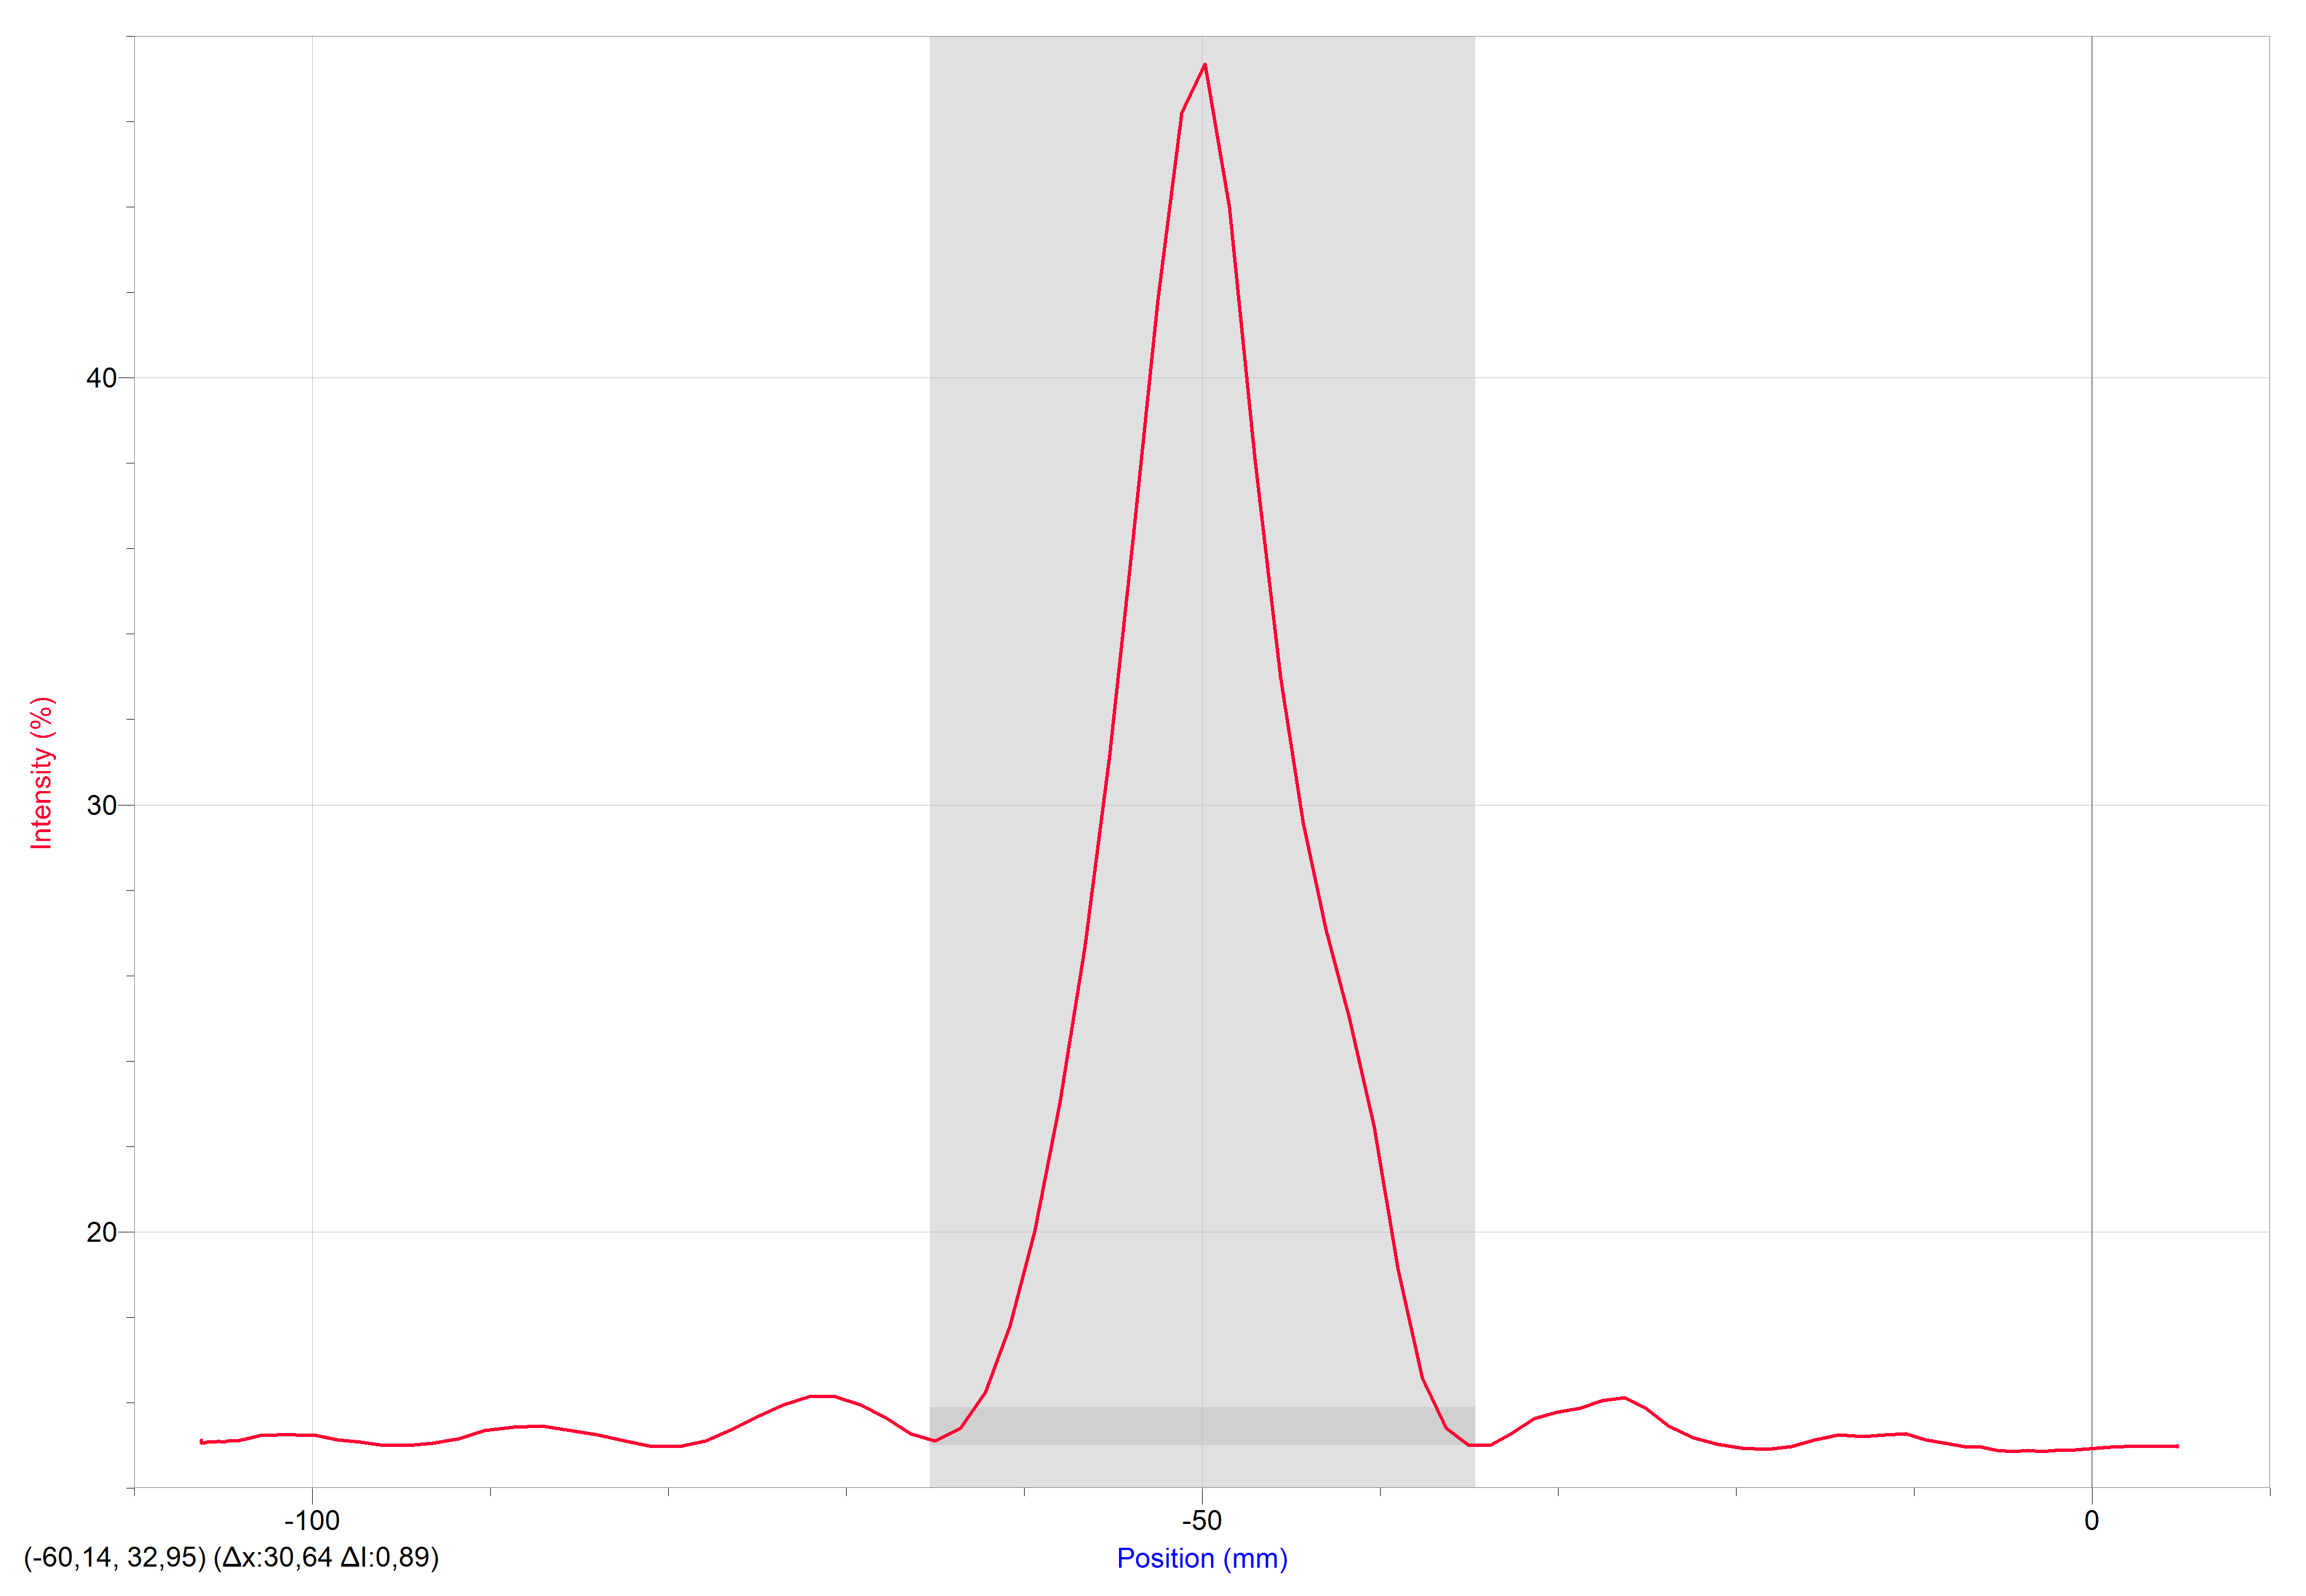
\includegraphics[width=0.94\textwidth]{RendijaAncha/DobleRendija004.png}
    \clearpage

    \item Rendija de \qty{0.08}{\mm}
    

    \begin{tabular}{|C|C|}
        \hline
        \text{Intensidad} (\%)    & \text{Posición} (\si{\mm})\\
        \hline
        15.7531738281      & -42.0369991725 \\
        17.3431396484      & -42.7143324925 \\
        21.9665527344      & -43.34933248   \\
        29.2495727539      & -43.941999135  \\
        39.192199707       & -44.53466579   \\
        50.7263183594      & -45.1696657775 \\
        62.956237793       & -45.804665765  \\
        75.8316040039      & -46.481999085  \\
        90.5715942383      & -47.159332405  \\
        99.9984741211      & -47.7943323925 \\
        99.9984741211      & -48.42933238   \\
        99.9984741211      & -49.021999035  \\
        99.9984741211      & -49.6569990225 \\
        99.9984741211      & -50.2496656775 \\
        \hline
    \end{tabular}
    \hspace{10pt}
    \begin{tabular}{|C|C|}
        \hline
        \text{Intensidad} (\%)    & \text{Posición} (\si{\mm})\\
        \hline
        99.9984741211      & -50.884665665  \\
        99.9984741211      & -51.47733232   \\
        99.9664306641      & -52.0276656425 \\
        84.407043457       & -52.5356656325 \\
        68.2495117188      & -53.085998955  \\
        52.3666381836      & -53.6363322775 \\
        38.4216308594      & -54.1866656    \\
        28.205871582       & -54.7369989225 \\
        21.8185424805      & -55.20266558   \\
        17.9901123047      & -55.625998905  \\
        16.0766601562      & -56.0916655625 \\
        15.5792236328      & -56.5149988875 \\
        \hline
    \end{tabular}

    $2 Y_0 = \qty{14.477999715}{\mm}$
    
    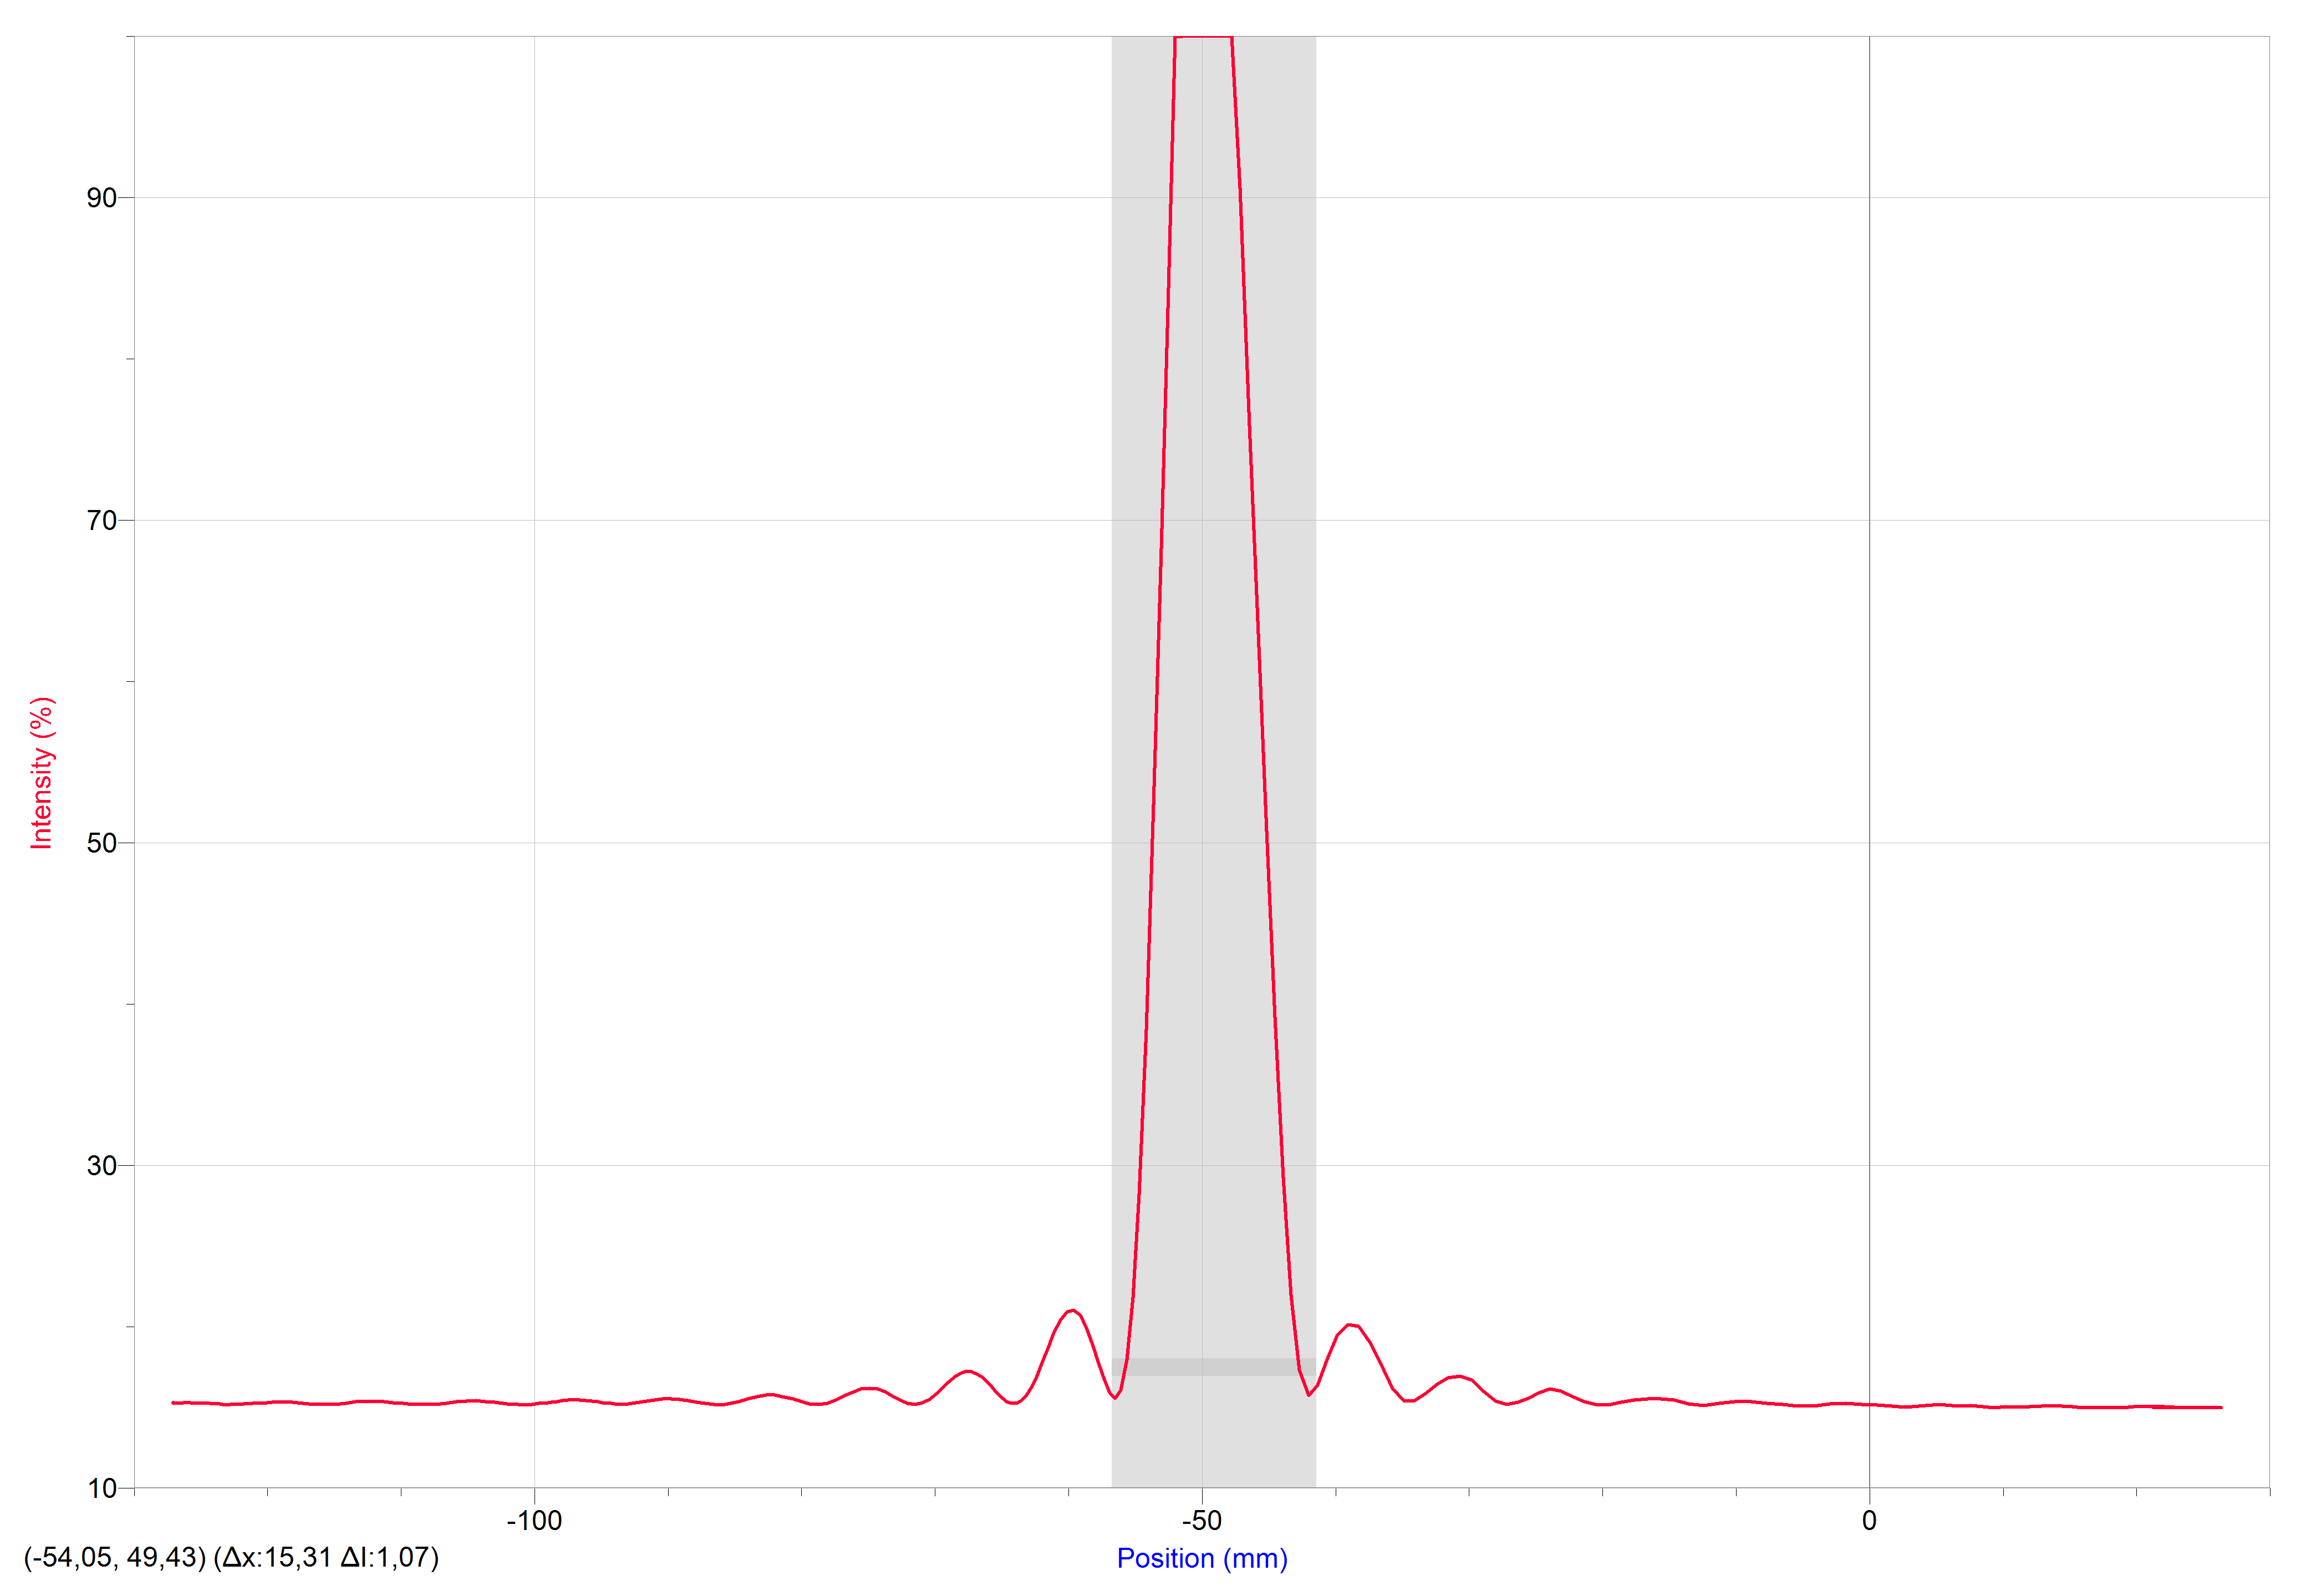
\includegraphics[width=0.94\textwidth]{RendijaAncha/DobleRendija008.png}
    % ~~~~ Aquí va imagen 0.08 ~~~~ %
    \clearpage
    \item Rendija de \qty{0.16}{\mm}
    
    \begin{tabular}{|C|C|}
        \hline
        \text{Intensidad} (\%)    & \text{Posición} (\si{\mm})\\
        \hline
        20.1278686523   & -45.465999105  \\
        34.5443725586   & -46.4396657525 \\
        99.9984741211   & -47.328665735  \\
        99.9984741211   & -48.1329990525 \\
        99.9984741211   & -48.8949990375 \\
        99.9984741211   & -49.5723323575 \\
        99.9984741211   & -50.2496656775 \\
        99.9984741211   & -50.884665665  \\
        99.9984741211   & -51.561998985  \\
        52.3910522461   & -52.2816656375 \\
        24.8748779297   & -52.9589989575 \\
        \hline
    \end{tabular}
    $2Y_0 = \qty{30,0143327425}{\mm}$

    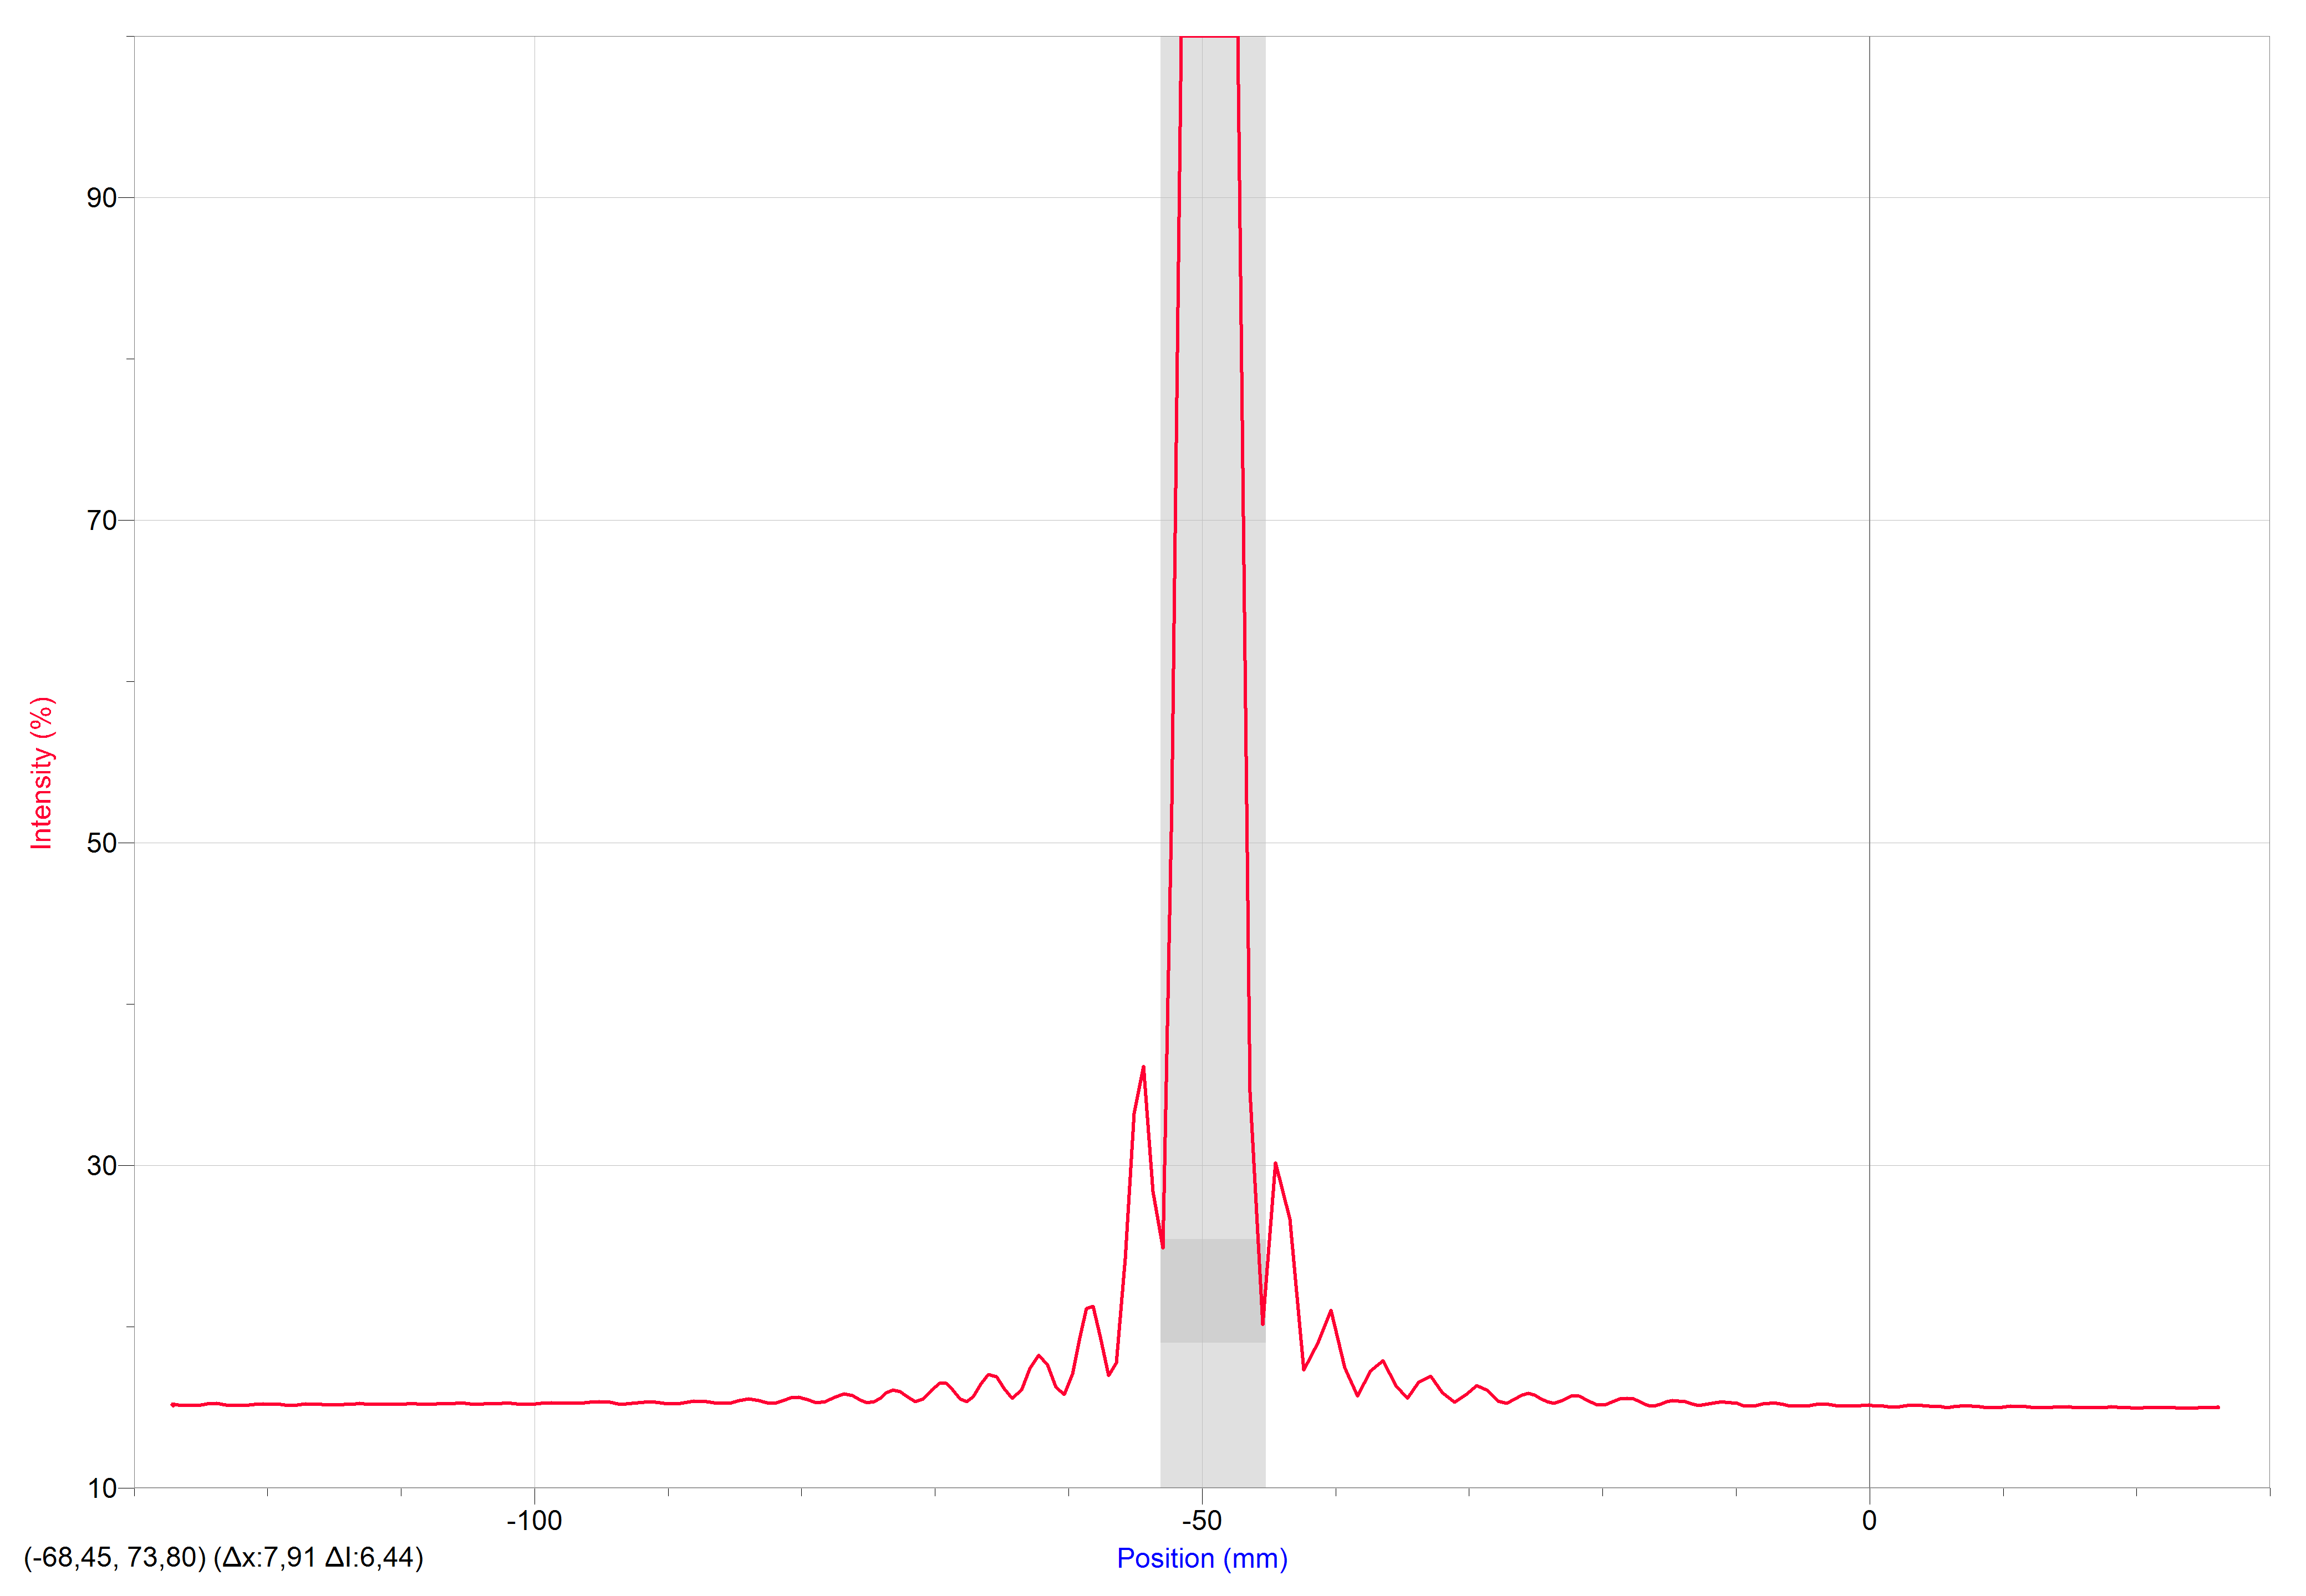
\includegraphics[width=0.94\textwidth]{RendijaAncha/RendijaAncha016.png}
    % ~~~~ Aquí va imagen 0.16 ~~~~ %
\end{enumerate}

\section{Resultados}
En los resultados se puede ver que en general, con el $Y_0$ encontrado
tanto manualmente como con el programa se puede aproximar
$\lambda$ a $6.35 \times 10^{-4}$ que es el $\lambda$ teórico. Entre
los experimentos hechos, el $\lambda$ hallado con la rendija de
$\SI{0.16}{\mm}$ a partir de la medida manual de $2Y_0 = \SI{8}{\mm}$
es el resultado más alejado del teórico con un error del 10\%; y el
valor más aproximado es el hallado con los datos del programa con la
rendija de $\SI{0.08}{\mm}$, donde $2Y_0 = \SI{14.478}{\mm}$, que
resutó en una longitud de onda
$\lambda = 6.363 \times 10^{-4}\ \si{\mm}$, con un error de
aproximación del 0.16\%

\end{document}